% !TEX root = Supplementary.tex
\documentclass[journal]{IEEEtran}
\bibliographystyle{IEEEtran}

\usepackage{amsmath,amsfonts,amssymb,amsthm,mathtools,mathrsfs}
\usepackage{nicefrac}
\usepackage{dsfont}
\usepackage{algorithm}
\usepackage{algorithmic}
\usepackage{multirow}
\usepackage{array}
\usepackage{booktabs}
\usepackage[caption=false,font=footnotesize,labelfont=rm,textfont=rm]{subfig}
\usepackage{textcomp}
\usepackage{stfloats}
\usepackage[hyphens]{url}
\usepackage{verbatim}
\usepackage{graphicx}
\usepackage{makecell}
\usepackage{cite}
\usepackage[table]{xcolor}
\usepackage{colortbl}
\usepackage{xspace}
\usepackage{balance}
\usepackage[colorlinks,
linkcolor=blue,
anchorcolor=blue,
citecolor=blue]{hyperref}
\usepackage{cleveref}



\newcommand{\x}{\mathbf{x}}
\newcommand{\z}{\mathbf{z}}
\newcommand{\y}{\mathbf{y}}
\newcommand{\w}{\mathbf{w}}
\newcommand{\data}{\mathcal{D}}
\DeclareMathOperator*{\E}{\mathbb{E}}

\newcommand{\etal}{{et~al.}\ }
\newcommand{\eg}{\emph{e.g.},\ }
\newcommand{\ie}{\emph{i.e.},\ }
\newcommand{\nth}{\text{th}}
\newcommand{\pr}{^\prime}
\newcommand{\tr}{^\mathrm{T}}
\newcommand{\inv}{^{-1}}
\newcommand{\pinv}{^{\dagger}}
\newcommand{\real}{\mathbb{R}}
\newcommand{\gauss}{\mathcal{N}}

\newcommand{\reward}{r}
\newcommand{\policy}{\pi}
\newcommand{\mdp}{\mathcal{M}}
\newcommand{\states}{\mathcal{S}}
\newcommand{\actions}{\mathcal{A}}
\newcommand{\observations}{\mathcal{O}}
\newcommand{\transitions}{T}
\newcommand{\initstate}{d_0}
\newcommand{\freq}{d}
\newcommand{\obsfunc}{E}
\newcommand{\initial}{\mathcal{I}}
\newcommand{\horizon}{H}
\newcommand{\rewardevent}{R}
\newcommand{\probr}{p_\rewardevent}
\newcommand{\metareward}{\bar{\reward}}
\newcommand{\discount}{\gamma}
\newcommand{\behavior}{{\pi_\beta}}
\newcommand{\bellman}{\mathcal{B}}
\newcommand{\qparams}{\phi}
\newcommand{\qparamset}{\Phi}
\newcommand{\qset}{\mathcal{Q}}
\newcommand{\batch}{B}
\newcommand{\qfeat}{\mathbf{f}}
\newcommand{\Qfeat}{\mathbf{F}}
\newcommand{\hatbehavior}{\hat{\pi}_\beta}

\newcommand{\traj}{\tau}

\newcommand{\pihi}{\pi^{\text{hi}}}
\newcommand{\pilo}{\pi^{\text{lo}}}
\newcommand{\ah}{\mathbf{w}}


\newcommand{\loss}{\mathcal{L}}
\newcommand{\eye}{\mathbf{I}}

\newcommand{\model}{\hat{p}}

\newcommand{\pimix}{\pi_{\text{mix}}}

\newcommand{\pib}{\bar{\pi}}
\newcommand{\epspi}{\epsilon_{\pi}}
\newcommand{\epsmodel}{\epsilon_{m}}

\newcommand{\return}{\mathcal{R}}

\newcommand{\cY}{\mathcal{Y}}
\newcommand{\cX}{\mathcal{X}}
\newcommand{\en}{\mathcal{E}}
\newcommand{\bu}{\mathbf{u}}
\newcommand{\bv}{\mathbf{v}}
\newcommand{\bd}{\mathbf{d}}
\newcommand{\be}{\mathbf{e}}
\newcommand{\by}{\mathbf{y}}
\newcommand{\ry}{\mathrm{y}}
\newcommand{\bx}{\mathbf{x}}
\newcommand{\bz}{\mathbf{z}}
\newcommand{\bw}{\mathbf{w}}
\newcommand{\boldm}{\mathbf{m}}
\newcommand{\bo}{\mathbf{o}}
\newcommand{\bs}{\mathbf{s}}
\newcommand{\ba}{\mathbf{a}}
\newcommand{\bM}{\mathbf{M}}
\newcommand{\ot}{\bo_t}
\newcommand{\st}{\bs_t}
\newcommand{\at}{\ba_t}
\newcommand{\op}{\mathcal{O}}
\newcommand{\opt}{\op_t}
\newcommand{\kl}{D_\text{KL}}
\newcommand{\tv}{D_\text{TV}}
\newcommand{\ent}{\mathcal{H}}
\newcommand{\bG}{\mathbf{G}}
\newcommand{\byk}{\mathbf{y_k}}
\newcommand{\bI}{\mathbf{I}}
\newcommand{\bg}{\mathbf{g}}
\newcommand{\bV}{\mathbf{V}}
\newcommand{\bD}{\mathbf{D}}
\newcommand{\bR}{\mathbf{R}}
\newcommand{\bQ}{\mathbf{Q}}
\newcommand{\bA}{\mathbf{A}}
\newcommand{\bN}{\mathbf{N}}
\newcommand{\bS}{\mathbf{S}}
\newcommand{\bW}{\mathbf{W}}
\newcommand{\bU}{\mathbf{U}}
\newcommand{\bO}{\mathbf{O}}
\newcommand{\leftnorm}{\left\vert \left\vert}
\newcommand{\rightnorm}{\right\vert \right\vert}

\newcommand{\bzhi}{\bz^\text{hi}}
\newcommand{\expected}{\mathbb{E}}
\newcommand{\deepnet}{\bW_N(k, t) \bW_\phi(k, t)}
\newcommand{\features}{\bW_\phi(k, t)}
\newcommand{\stateactioni}{[\bs_i; \ba_i]}
\newcommand{\cosine}{\text{cos}}


\def\thetaP{\theta^{\prime}}
\def\cf{\emph{c.f.}\ }
\def\vs{\emph{vs}.\ }
\def\etc{\emph{etc.}\ }
\def\Eqref#1{Equation~\ref{#1}}
\def\ss#1{\scriptsize #1}

\newenvironment{repeatedthm}[1]{\@begintheorem{#1}{\unskip}}{\@endtheorem}

\newcommand{\methodname}{Cal-QL}
\newcommand{\aliasingproblemname}{bootstrapping aliasing}
\newcommand{\Aliasingproblemname}{Bootstrapping aliasing}
\newcommand{\AliasingProblemName}{Bootstrapping Aliasing}
\newcommand{\simnorm}{\mathrm{sim}_{\mathrm{n}}^\pi}
\newcommand{\simunnorm}{\mathrm{sim}_{\mathrm{u}}^\pi}

\definecolor{blanchedalmond}{rgb}{1.0, 0.92, 0.8}
\definecolor{carmine}{rgb}{0.59, 0.0, 0.09}
\definecolor{lightblue}{rgb}{0.22,0.45,0.70}



\newcommand{\rebuttal}[1]{#1}
\newcommand{\scenario}[1]{\textcolor{lightblue}{S#1}}
\newcommand{\technique}[1]{\textcolor{carmine}{T#1}}
\newcommand{\application}[1]{\textcolor{carmine}{A#1}}

\def\bellmanop{T^\circ}
\def\qop{Q^\circ}
\def\qpi{Q^\pi}
\def\qs{Q^*}
\def\Qstar{Q^*}
\def\Qt{Q_{\theta}}
\def\Qtp{Q_{\thetaP}}
\def\ld{\ell_{\lambda}}



\newtheorem{theorem}{Theorem}[section]
\newtheorem{sketchtheorem}{Sketch Theorem}[section]
\newtheorem{lemma}[theorem]{Lemma}
\newtheorem{corollary}[theorem]{Corollary}
\newtheorem{proposition}[theorem]{Proposition}
\newtheorem{definition}[theorem]{Definition}
\newtheorem{conjecture}[theorem]{Conjecture}
\newtheorem{problem}[theorem]{Problem}
\newtheorem{formulation}[theorem]{Formulation}
\newtheorem{claim}[theorem]{Claim}
\newtheorem{remark}[theorem]{Remark}
\newtheorem{example}[theorem]{Example}
\newtheorem{assumption}[theorem]{Assumption}
\newtheorem{exercise}[theorem]{Exercise}


\newcommand{\indep}{\rotatebox[origin=c]{90}{$\models$}}

\renewcommand{\mathbf}{\boldsymbol}

\newcommand{\conv}{\circledast}
\newcommand{\mb}{\mathbf}
\newcommand{\mc}{\mathcal}
\newcommand{\mf}{\mathfrak}
\newcommand{\md}{\mathds}
\newcommand{\bb}{\mathbb}
\newcommand{\msf}{\mathsf}
\newcommand{\mcr}{\mathscr}
\newcommand{\magnitude}[1]{ \left| #1 \right| }
\newcommand{\set}[1]{\left\{ #1 \right\}}
\newcommand{\condset}[2]{ \left\{ #1 \;\middle|\; #2 \right\} }


\newcommand{\reals}{\bb R}
\newcommand{\proj}{\mathrm{proj}}

\newcommand{\eps}{\varepsilon}
\newcommand{\R}{\reals}
\newcommand{\Cp}{\bb C}
\newcommand{\Z}{\bb Z}
\newcommand{\N}{\bb N}
\newcommand{\Sp}{\bb S}
\newcommand{\Ba}{\bb B}
\newcommand{\indicator}[1]{\mathbbm 1\left\{#1\right\}}
\renewcommand{\P}{\mathbb{P}}
\newcommand{\rvline}{\hspace*{-\arraycolsep}\vline\hspace*{-\arraycolsep}}
\makeatletter
\def\Ddots{\mathinner{\mkern1mu\raise\p@
\vbox{\kern7\p@\hbox{.}}\mkern2mu
\raise4\p@\hbox{.}\mkern2mu\raise7\p@\hbox{.}\mkern1mu}}
\makeatother


\newcommand{\event}{\mc E}

\newcommand{\e}{\mathrm{e}}
\newcommand{\im}{\mathrm{i}}
\newcommand{\rconcave}{r_\fgecap}
\newcommand{\Lconcave}{\mc L^\fgecap}
\newcommand{\rconvex}{r_\fgecup}
\newcommand{\Rconvex}{R_\fgecup}
\newcommand{\Lconvex}{\mc L^\fgecup}

\newcommand{\wh}{\widehat}
\newcommand{\wt}{\widetilde}
\newcommand{\ol}{\overline}


\newcommand{\betaconcave}{\beta_\fgecap}
\newcommand{\betagrad}{\beta_{\mathrm{grad}}}

\newcommand{\norm}[2]{\left\| #1 \right\|_{#2}}
\newcommand{\abs}[1]{\left| #1 \right|}
\newcommand{\row}[1]{\text{row}\left( #1 \right)}
\newcommand{\innerprod}[2]{\left\langle #1,  #2 \right\rangle}
\newcommand{\prob}[1]{\bb P\left[ #1 \right]}
\newcommand{\expect}[1]{\bb E\left[ #1 \right]}
\newcommand{\function}[2]{#1 \left(#2\right}
\newcommand{\integral}[4]{\int_{#1}^{#2}\; #3\; #4}
\newcommand{\paren}[1]{\left( #1 \right)}
\newcommand{\brac}[1]{\left[ #1 \right]}
\newcommand{\Brac}[1]{\left\{ #1 \right\}}

\newcommand{\moff}{m_\mr{off}}
\newcommand{\mon}{m_\mr{on}}
\newcommand{\EmpiricalOffline}{\wh{\bb E}_{\mc D^\nu_h}}
\newcommand{\EmpiricalOnline}{\wh{\bb E}_{\mc D^\tau_h}}
\newcommand{\Deltaoff}{\Delta_\mr{off}}
\newcommand{\Deltaon}{\Delta_\mr{on}}
\newcommand{\Vmax}{V_{\max}}
\newcommand{\regret}{\mr{Reg}}
\newcommand{\regreton}{\mr{Sub}_{\mr {on}}}
\newcommand{\regretoff}{\mr{Sub}_{\mr {off}}}
\newcommand{\Doff}{\mc D_\mr{off}}
\newcommand{\Don}{\mc D_\mr{on}}
\newcommand{\piref}{\pi_\mr{ref}}


\newcommand{\mr}{\mathrm}
\newcommand{\sym}{\mathrm{Sym}}
\newcommand{\sks}{\mathrm{Skew}}
\newcommand{\inprod}[2]{\langle#1,#2\rangle}
\newcommand{\parans}[1]{\left(#1\right}
\newcommand{\clip}{\msf{clipped}}
\newcommand{\beha}{\msf b}

\definecolor{amaranth}{rgb}{0.9, 0.17, 0.31}
\definecolor{antiquebrass}{rgb}{0.8, 0.58, 0.46}
\definecolor{antiquefuchsia}{rgb}{0.57, 0.36, 0.51}
\definecolor{chromeyellow}{rgb}{0.31, 0.47, 0.26}
\newcommand{\sft}{\mathrm{sft}}
\newcommand{\negtext}{\text{neg}}

\newcommand{\hatby}{\hat{\by}}

\newcommand{\rftdata}{\mathcal{D}^+_{\pi_\sft}}
\newcommand{\dpodata}{\mathcal{D}^{\pm}_{\pi_\sft}}
\newcommand{\syndata}{\mathcal{D}_{\mathrm{syn}}}

\newcommand{\posby}{+\by}
\newcommand{\negby}{-\by}
\newcommand{\hatposby}{+\hat{\by}}
\newcommand{\hatnegby}{-\hat{\by}}



\newcommand{\bok}{\text{BoK}}

\def \endprf{\hfill {\vrule height6pt width6pt depth0pt}\medskip}



\newcommand{\lzone}{l_{0-1}}
\newcommand{\brck}[1]{\left [ #1 \right ] }

\newcommand{\faft}{\mathrm{fa-ft}}
\newcommand{\bfC}{\mathbf{C}}
\newcommand{\bP}{\mathbf{P}}

\newcommand{\inlinegraphicorfallback}[4]{%
  \IfFileExists{#2}{\raisebox{-1.5pt}{\includegraphics[#1]{#2}}}{%
    \IfFileExists{#3}{\raisebox{-1.5pt}{\includegraphics[#1]{#3}}}{#4}}%
}
\newcommand{\github}{\inlinegraphicorfallback{height=1.05em}{Figures/github-logo.pdf}{figures/github-logo.pdf}{GitHub}}
\newcommand{\wnb}{\inlinegraphicorfallback{height=1.05em}{Figures/wnb-logo.jpeg}{figures/wnb-logo.jpeg}{W\&B}}
\newcommand{\paperlogo}{\inlinegraphicorfallback{height=2.05em}{Figures/paper-logo.png}{figures/paper-logo.png}{SG-WAM}}

% Method name
\usepackage{xspace}
\newcommand{\ourmethod}{SG-WAM\xspace}
% !TEX root = AnonymousSubmission2027.tex

\renewcommand{\paragraph}[1]{\par\vspace{0.35em}\noindent\textbf{#1}\quad}

\title{Supplementary Material for ``SG-WAM: Text-Grounded and Spatial-Aware Semantic Guidance for World-Action Models''}
\author{Junjie He, Co-Author Name, and Corresponding Author}

\begin{document}

\maketitle

% !TEX root = ../AnonymousSubmission2027.tex

\section{Additional Implementation Details}
\label{sec:appendix_impl}

\paragraph{Semantic Planner.}
The planner is a Qwen3.5 2B~\cite{qwen35} backbone that receives one camera view, the language
instruction, and the learnable query tokens in a single multimodal sequence.
Each future keyframe is represented by $32$ shared base tokens together with $32$ modality-specific tokens per branch, so a keyframe contributes $96$ query positions in total.
The two resampler heads share the same architecture and differ only in their output width, which matches the feature dimension of the corresponding
semantic foresight representation ($1024$ for the text-grounded branch and
$2048$ for the spatial-aware branch).
The planner is applied to every camera view with shared weights, and the per-view predictions are concatenated before they enter the world-action model.

\paragraph{Semantic Foresight Representations.}
Both representation encoders are frozen and run in inference mode.
The target representations are computed online for every training batch rather
than cached, so that they always match the augmentation applied to the input
frames.
For SigLIP2~\cite{siglip2} we take the penultimate-layer patch tokens, and for
Depth Anything~3~\cite{lin2025depth} we take the last-layer dense features.
Neither encoder is used at inference, where the planner alone supplies the
guidance.

\paragraph{World-Action Model.}
The world-action model follows a mixture-of-transformers (MoT) design: the video
expert and the action expert are two parallel transformer streams with separate
parameters, and in every block their tokens are concatenated into a single
sequence for joint attention before returning to expert-specific cross-attention
and feed-forward layers.
This joint attention is the only place where the two streams interact, and it is
how the action tokens read the guidance: the semantic guidance is injected only
into the video expert, and the action expert inherits it by attending to the
guided video tokens.
The video expert is initialized from a pretrained LTX-Video~\cite{ltxvideo} diffusion model with
$28$ transformer blocks, and we insert the guidance cross-attention into every
block alongside the original text cross-attention with a zero-initialized gate.
The action expert mirrors the block structure of the video expert, receives the
robot state, and denoises the action chunk with the same flow-matching
formulation as the video branch.
The model consumes the current observation together with recent context frames
and generates $T{=}9$ future frames at $256{\times}256$ and an action chunk of
$H{=}36$ steps per planner call, so the guidance is refreshed once per chunk
rather than at every control step.

\paragraph{Optimization.}
All stages use AdamW with gradient clipping at $1.0$ and bf16 mixed precision,
sharded across eight H100 GPUs with ZeRO stage~2.
Stage~1 follows a cosine schedule, while Stages~2 and~3 keep the learning rate
constant after warmup so that the pretrained video prior is perturbed as little
as possible once the guidance branch starts to contribute.
The guidance-dropout probability is $0.15$ in every stage that involves the
world-action model.

\paragraph{Planner Input Format.}
Each planner call is a single-turn chat sequence that contains one camera image,
the text ``Instruction: $\langle$instruction$\rangle$'', and a plan region
delimited by \texttt{<PLAN\_START>} and \texttt{<PLAN\_END>}.
Inside this region, a frame marker \texttt{<FRAME\_k>} introduces the query
tokens of the $k$-th future keyframe, and the hidden states at these positions
are read out as the planner's prediction.
Each camera view forms its own sequence with a shared copy of the instruction,
and the per-view sequences are processed in a single batch with shared weights.

\paragraph{Inference Details.}
At inference, the planner runs once per action chunk: a single forward pass
produces the guidance for all $K{=}4$ keyframes and both views.
Conditioned on this guidance, the video and action experts denoise with $10$
Euler steps of the flow-matching sampler, and the semantic guidance is applied
at every denoising step.
The policy executes the first $8$ of the $36$ predicted actions and then
re-plans in a receding-horizon manner, so one planner and world-action forward
pass is amortized over eight control steps.

\section{Benchmark and Data Details}
\label{sec:appendix_tasks}

\begin{figure*}[t]
    \centering
    % Generated by scripts/plot_supp_rollout.py; edit HEIGHT and re-run to swap videos.
    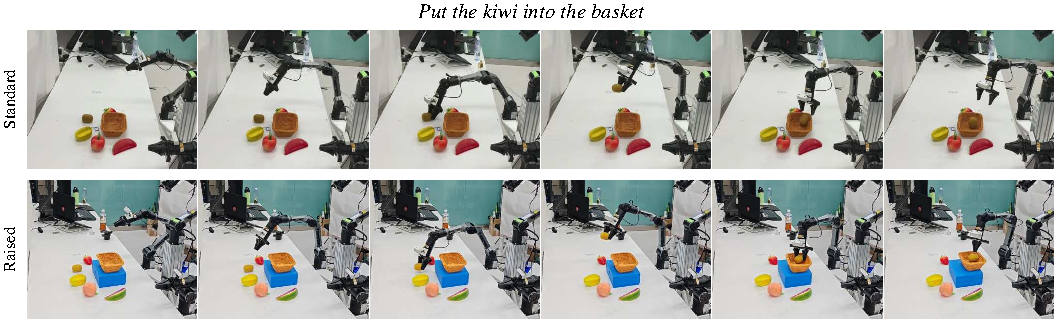
\includegraphics[width=\textwidth]{Figures/supp_height.pdf}
    \caption{\textbf{Rollouts at the standard and the unseen container
    height.} Keyframes of \ourmethod on the basket task with the container on
    the table as in the demonstrations (top) and raised on a platform that
    never appears in the demonstrations (bottom). The policy adjusts the
    lifting and placing motion to the new height and completes the task in both
    cases.}
    \label{fig:supp_height}
\end{figure*}

\begin{table*}[t]
\centering
\begingroup
\small
\setlength{\tabcolsep}{6pt}
\begin{tabular*}{0.78\textwidth}{@{\extracolsep{\fill}}lccccc}
\toprule
Variant & Spatial & Object & Goal & Long & Avg \\
\midrule
\ourmethod (full) & \textbf{99.4} & \textbf{99.4} & \textbf{98.2} & \textbf{97.8} & \textbf{98.7} \\
\midrule
\multicolumn{6}{l}{\textit{Semantic guidance}} \\
\quad w/o semantic guidance & 98.6 & 97.8 & 96.6 & 95.8 & 97.2 \\
\multicolumn{6}{l}{\textit{Dual-semantics design}} \\
\quad w/o spatial-aware semantics & 98.6 & 99.2 & 98.0 & 97.4 & 98.3 \\
\quad w/o text-grounded semantics & 99.0 & 98.0 & 96.8 & 97.0 & 97.7 \\
\quad w/o shared semantic query tokens & 99.2 & 99.0 & 97.8 & 97.6 & 98.4 \\
\multicolumn{6}{l}{\textit{Three-stage training}} \\
\quad single-stage training & 99.0 & 98.8 & 97.4 & 96.4 & 97.9 \\
\bottomrule
\end{tabular*}
\endgroup
\caption{
Per-suite success rates (\%) on LIBERO for the ablated variants.
The Avg column matches the ablation table in the main paper.
Bold indicates the best result.
}
\label{tab:appendix_ablation_detail}
\end{table*}

\begin{figure*}[t]
    \centering
    % Generated by scripts/plot_supp_rollout.py; edit LIGHT and re-run to swap videos.
    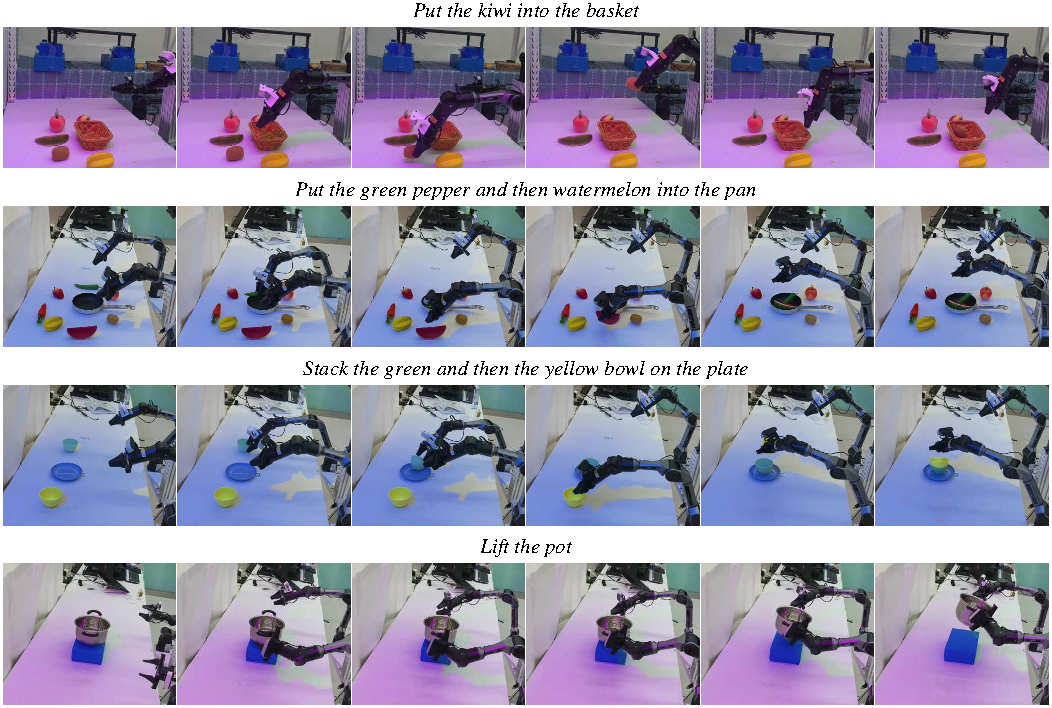
\includegraphics[width=\textwidth]{Figures/supp_light.pdf}
    \caption{\textbf{Rollouts under unseen colored lighting.} Keyframes of
    \ourmethod on all four tasks under lighting conditions that differ from data
    collection. The policy still selects the instructed objects and completes
    each task.}
    \label{fig:supp_light}
\end{figure*}


\paragraph{Simulation Benchmark.}
We evaluate on two simulation benchmarks:
\begin{itemize}
    \item \textbf{LIBERO}~\cite{liu2023libero} contains four suites (Spatial,
    Object, Goal, and Long) of ten tabletop manipulation tasks each.
    Following the standard protocol, we evaluate $500$ trials per suite and
    report the success rate.
    \item \textbf{LIBERO-Plus}~\cite{liberoplus} perturbs the original LIBERO
    tasks along seven factors, covering object layout, camera viewpoint, robot
    initial state, language rephrasing, lighting, background texture, and
    sensor noise.
    We use the released perturbation suites without modification, so that our
    numbers are directly comparable to the published baselines, and we report
    the success rate over all perturbed tasks.
\end{itemize}

\paragraph{Real-World Platform.}
The platform is an AgileX Cobot with two 6-DoF Piper arms, each equipped with a
1-DoF parallel gripper, so the observation and action are both
$14$-dimensional (six joints and one gripper per arm).
Three Orbbec Dabai DC1 cameras provide the visual input, one front-facing
camera as Eye-on-Base and one on each wrist as Eye-on-Hand, all recording
$640{\times}480$ RGB at $30$\,fps; depth is not used.
Demonstrations are collected through master--puppet teleoperation at
$30$\,Hz, which is also the time axis of the recorded observations and
actions, while the low-level arm controller runs at $200$\,Hz.
Each task is recorded with $100$ teleoperated demonstrations and evaluated over
$50$ trials per method, with object positions re-randomized between trials.
The two generalization settings reuse the same policies without any fine-tuning:
the basket task is repeated with the container raised to a height that never
appears in the demonstrations, and the pan task is repeated under colored
lighting that differs from the data-collection condition.

\paragraph{Real-World Baselines.}
GE-Act and FastWAM are fine-tuned on the same $100$ demonstrations per task as
\ourmethod and receive the same camera views as input.
Each baseline keeps the action-chunk configuration of its official release, and
FastWAM follows the setting used for its RoboTwin experiments, which matches
our dual-arm platform.
All remaining hyperparameters follow the official recipes of the respective
baselines, so the comparison differs only in the conditioning of generation.



\section{Ablation Variant Details}
\label{sec:appendix_ablation}

All ablated variants in the main paper are trained with the same data, batch
size, schedules, and number of steps as the full model; only the component
under study changes.
\begin{itemize}
    \item \textbf{w/o semantic guidance} removes the semantic planner and the
    guidance cross-attention branch entirely, so the world-action model is
    conditioned on the text embedding alone, matching the plain text-conditioned
    baseline built on the same backbone.
    \item \textbf{w/o text-grounded semantics} and
    \textbf{w/o spatial-aware semantics} each drop one branch: the
    corresponding resampler head, alignment term, and projection in the fusion
    are removed, and the guidance reduces to the remaining branch.
    The query tokens of the removed branch are also removed, while the shared
    base tokens are kept.
    \item \textbf{w/o shared semantic query tokens} replaces the base group
    with additional branch-private tokens so that the total number of query
    tokens per keyframe is unchanged, isolating the effect of sharing rather
    than that of capacity.
    \item \textbf{single-stage training} skips Stages~1 and~2: the planner,
    the world model, and the action expert are initialized in the same way and
    optimized jointly from scratch for the same total number of steps under the
    Stage-3 objective.
\end{itemize}

Table~\ref{tab:appendix_ablation_detail} breaks the ablation down by LIBERO
suite.
Removing the text-grounded semantics hurts most on the Object and Goal suites,
where the instructed target has to be identified, whereas removing the
spatial-aware semantics hurts most on the Spatial suite, matching the intended
roles of the two branches.
Removing the guidance entirely and skipping the staged training degrade most on
the Long suite, where errors accumulate over the horizon.


\section{Additional Real-World Visualizations}
\label{sec:appendix_vis}


Figures~\ref{fig:supp_height} and~\ref{fig:supp_light} visualize additional
real-world rollouts under the two generalization settings.
In Figure~\ref{fig:supp_height}, the same policy is shown at the standard
container height and with the basket raised on a platform that never appears in
the demonstrations, and \ourmethod adapts the grasp height and the placing
motion accordingly.
In Figure~\ref{fig:supp_light}, the workspace is lit in colors that differ
from the data-collection condition; across all four tasks the policy still
grounds the instruction on the correct objects, which is consistent with the
lighting robustness observed on LIBERO-Plus.



\bibliography{references}

\end{document}
